%%%%%%%%%%%%%%%%%%%%%%%%%%%%%%%%%%%%%%%%%
% Dreuw & Deselaer's Poster
% LaTeX Template
% Version 1.0 (11/04/13)
%
% Created by:
% Philippe Dreuw and Thomas Deselaers
% http://www-i6.informatik.rwth-aachen.de/~dreuw/latexbeamerposter.php
%
% This template has been downloaded from:

% http://www.LaTeXTemplates.com
%
% License:
% CC BY-NC-SA 3.0 (http://creativecommons.org/licenses/by-nc-sa/3.0/)
%
%%%%%%%%%%%%%%%%%%%%%%%%%%%%%%%%%%%%%%%%%

%----------------------------------------------------------------------------------------
%	PACKAGES AND OTHER DOCUMENT CONFIGURATIONS
%----------------------------------------------------------------------------------------

\documentclass[final,hyperref={pdfpagelabels=false}]{beamer}

\usepackage[orientation=portrait,size=a0,scale=1.4]{beamerposter} % Use the beamerposter package for laying out the poster with a portrait orientation and an a0 paper size
\usepackage[backend=biber,maxbibnames=9]{biblatex}
\addbibresource{bibliography.bib}
\usetheme{I6pd2} % Use the I6pd2 theme supplied with this template

\usepackage[english]{babel} % English language/hyphenation

\usepackage{amsmath,amsthm,amssymb,latexsym} % For including math equations, theorems, symbols, etc

%\usepackage{times}\usefonttheme{professionalfonts}  % Uncomment to use Times as the main font
%\usefonttheme[onlymath]{serif} % Uncomment to use a Serif font within math environments

\boldmath % Use bold for everything within the math environment

\usepackage{booktabs} % Top and bottom rules for tables

\graphicspath{{figures/}} % Location of the graphics files

\usecaptiontemplate{\small\structure{\insertcaptionname~\insertcaptionnumber: }\insertcaption} % A fix for figure numbering

%----------------------------------------------------------------------------------------
%	TITLE SECTION 
%----------------------------------------------------------------------------------------

\title{\huge Structural Identifiability via the Web App:\\A Maple Cloud Toolbox} % Poster title

\author{John Smith, James Smith and Jane Smith} % Author(s)

\institute{Department and University Name} % Institution(s)

%----------------------------------------------------------------------------------------
%	FOOTER TEXT
%----------------------------------------------------------------------------------------

\newcommand{\leftfoot}{https://iliailmer.github.io} % Left footer text

\newcommand{\rightfoot}{john@smith.com} % Right footer text

%----------------------------------------------------------------------------------------

\begin{document}

\addtobeamertemplate{block end}{}{\vspace*{2ex}} % White space under blocks

\begin{frame}[t] % The whole poster is enclosed in one beamer frame

    \begin{columns}[t] % The whole poster consists of two major columns, each of which can be subdivided further with another \begin{columns} block - the [t] argument aligns each column's content to the top

        \begin{column}{.02\textwidth}\end{column} % Empty spacer column

        \begin{column}{.465\textwidth} % The first column

            %----------------------------------------------------------------------------------------
            %	OBJECTIVES
            %----------------------------------------------------------------------------------------

            \begin{block}{Introduction}

                \begin{enumerate}
                    \item Structural parameter identifiability describes whether a parameter value can be recovered from data before performing experiments.
                    \item A parameter is can be \emph{locally} (finitely many values) or \emph{globally} (uniquely) identifiable.
                    \item If neither is the case, we say that a parameter is unidentifiable and we seek \emph{identifiable combinations} (functions of parameters that are globally identifiable).
                    \item Some parameters may be identifiable from more than one experiment. Finding the bound on the maximal amount of experiments is crucial.
                \end{enumerate}

            \end{block}

            %----------------------------------------------------------------------------------------
            %	INTRODUCTION
            %----------------------------------------------------------------------------------------

            \begin{block}{Motivating Examples}

                \begin{itemize}
                    \item {\bf A simple two-parameter model} \begin{equation}
                              \begin{cases}
                                  x' = A^2, \\
                                  x(0) = B, \\
                                  y = x
                              \end{cases}\Rightarrow\begin{cases}
                                  %   \text{Solution: } x = A^2t+B, \\
                                  \text{Globally: } B=y(0), \\
                                  \text{Locally: }A=\pm\sqrt{y(1)-y(0)}
                              \end{cases}
                          \end{equation}
                    \item {\bf Unidentifiable case}\begin{equation}
                              \begin{cases}
                                  x' = 0, \\
                                  y_1 = x,~y_2=Cx+D
                              \end{cases}\Rightarrow\begin{cases}
                                  \text{Globally: } x(0)=y(0) \\
                                  \text{Unidentifiable: } C, D
                              \end{cases}
                          \end{equation}
                    \item The latter case is mitigated by performing \emph{2 experiments:}
                          \begin{equation}
                              \begin{cases}
                                  x_1' = 0,~x_2'=0            \\
                                  y_{11} = x_1,~y_{12}=Cx_1+D \\
                                  y_{21} = x_2,~y_{22}=Cx_2+D \\
                              \end{cases}\Rightarrow\begin{cases}
                                  \text{Globally: } C, D
                              \end{cases}
                          \end{equation}
                \end{itemize}

            \end{block}

            %----------------------------------------------------------------------------------------
            %	MATERIALS
            %----------------------------------------------------------------------------------------

            \begin{block}{Web Based Identifiability Toolbox \cite{ilmer_web-based_2021}}

                \begin{itemize}
                    \item All-in-one solution available at \url{https://maple.cloud/app/6509768948056064/}
                    \item Implements algorithms for individual parameters' global identifiability \cite{hong_sian_2019}.
                    \item Capable of finding \emph{single-} and \emph{multi-}experiment identifiable combinations of parameters according \cite{ovchinnikov2020computing,ovchinnikov2020multi}.
                    \item We will refer to these identifiability types as SE and ME, respectively.
                \end{itemize} % End of the subdivision

                % The algorithms included in the toolbox 
            \end{block}

            %----------------------------------------------------------------------------------------
            %	METHODS
            %----------------------------------------------------------------------------------------

            \begin{block}{Input Format}

                \begin{itemize}
                    \item Both individual parameter identifiability and identifiable combinations algorithms accept the same input format:
                          \[\Sigma:=\begin{cases}
                                  \mathbf{x}'=\mathbf{f}(\mathbf{x},\boldsymbol{\mu}, \mathbf{u}), \\
                                  \mathbf{y}=\mathbf{g}(\mathbf{x}, \boldsymbol{\mu}, \mathbf{u}).
                              \end{cases}\]
                          \(\mathbf{f}=(f_1, \dots, f_n)\) and \(\mathbf{g}=(g_1,\dots,g_n)\) are tuples of rational functions with coefficients in \(\mathbb{C}\). Here \(\mathbf{x}, \boldsymbol{\mu}, \mathbf{y}, \mathbf{u}\) are states, parameters, outputs, and inputs, respectively.
                    \item Individual parameter results are guaranteed with user-fixed probability of correctness (0.99 by default)
                    \item The combination-wise result is deterministic.
                    \item Lengthy symbolic computing can be sped up via individual parameter \emph{bypass}: if all parameters are globally identifiable we treat them as trivial identifiable combinations
                \end{itemize}

            \end{block}
            \begin{block}{Table: Timings}

                \begin{itemize}
                    \item Timing of built-in ODE examples
                \end{itemize}
                \begin{table}[htbp] % h:here; t:top; b:bottom; p:page; default:ht
                    \centering
                    \begin{tabular}{lccc}
                        \hline
                        Name                                             & SIAN & ME    & SE                  \\\hline\hline
                        {\tt Biohydrogenation}                           & 3.8  & 160.9 & 160.9               \\
                        {\tt Treatment}                                  & 2.7  & 1.5   & 1.5                 \\
                        {\tt Tumor}                                      & 6.8  & 0.0   & 0.0                 \\
                        {\tt Chemical Reaction Network}                  & 6.0  & 0.0   & 0.0\footnotemark[8] \\
                        {\tt Chemical Reaction Network} (without bypass) & 5.0  & 390.2 & 390.2               \\
                        \hline
                    \end{tabular}
                    \caption{CPU Times with bypass for some of the built-in examples}
                    \label{tab:def}
                \end{table}

            \end{block}

            %----------------------------------------------------------------------------------------
            %	MATHEMATICAL SECTION
            %----------------------------------------------------------------------------------------

            % \begin{block}{Mathematical Section}

            %     \begin{itemize}
            %         \item Maecenas Ultricies Feugiat Velit Non Mattis.
            %               \begin{itemize}
            %                   \item Duis ante erat, bibendum nec tempus nec, interdum quis est. Nulla at mollis tortor. Phasellus quis leo dolor, aliquam laoreet orci $X$ Donec dapibus sagittis neque eu nec, interdum quis est. $Y_n, n=1,\cdots,N$ ndum nec tempus nec, interd
            %                         \begin{align*}
            %                             X \rightarrow r(X) & = \arg \max_{c} \Big\{ \max_n \big\{ \sum_{x_i \in X} \delta(x_i,Y_{n,c})\big\} \Big\}
            %                         \end{align*}
            %                   \item Cras faucibus scelerisque cursus. Proin ut vestibulum augue. $\delta(x_i,Y_{n,c})$
            %               \end{itemize}
            %         \item Fusce tempus arcu id ligula varius dictum. Donec ut nisl dui, ac consectetur elit. In nec enim porta augue venenatis sollicitudin. Phasellus quis nunc neque. Suspendisse mauris diam, suscipit non gravida in, placerat id enim. Ut nec ipsum in lectus ultrices sagittis.
            %     \end{itemize}

            % \end{block}

            %----------------------------------------------------------------------------------------

        \end{column} % End of the first column

        \begin{column}{.03\textwidth}\end{column} % Empty spacer column

        \begin{column}{.465\textwidth} % The second column

            %----------------------------------------------------------------------------------------
            %	RESULTS
            %----------------------------------------------------------------------------------------



            %------------------------------------------------

            \begin{block}{Screenshot}

                \begin{figure}
                    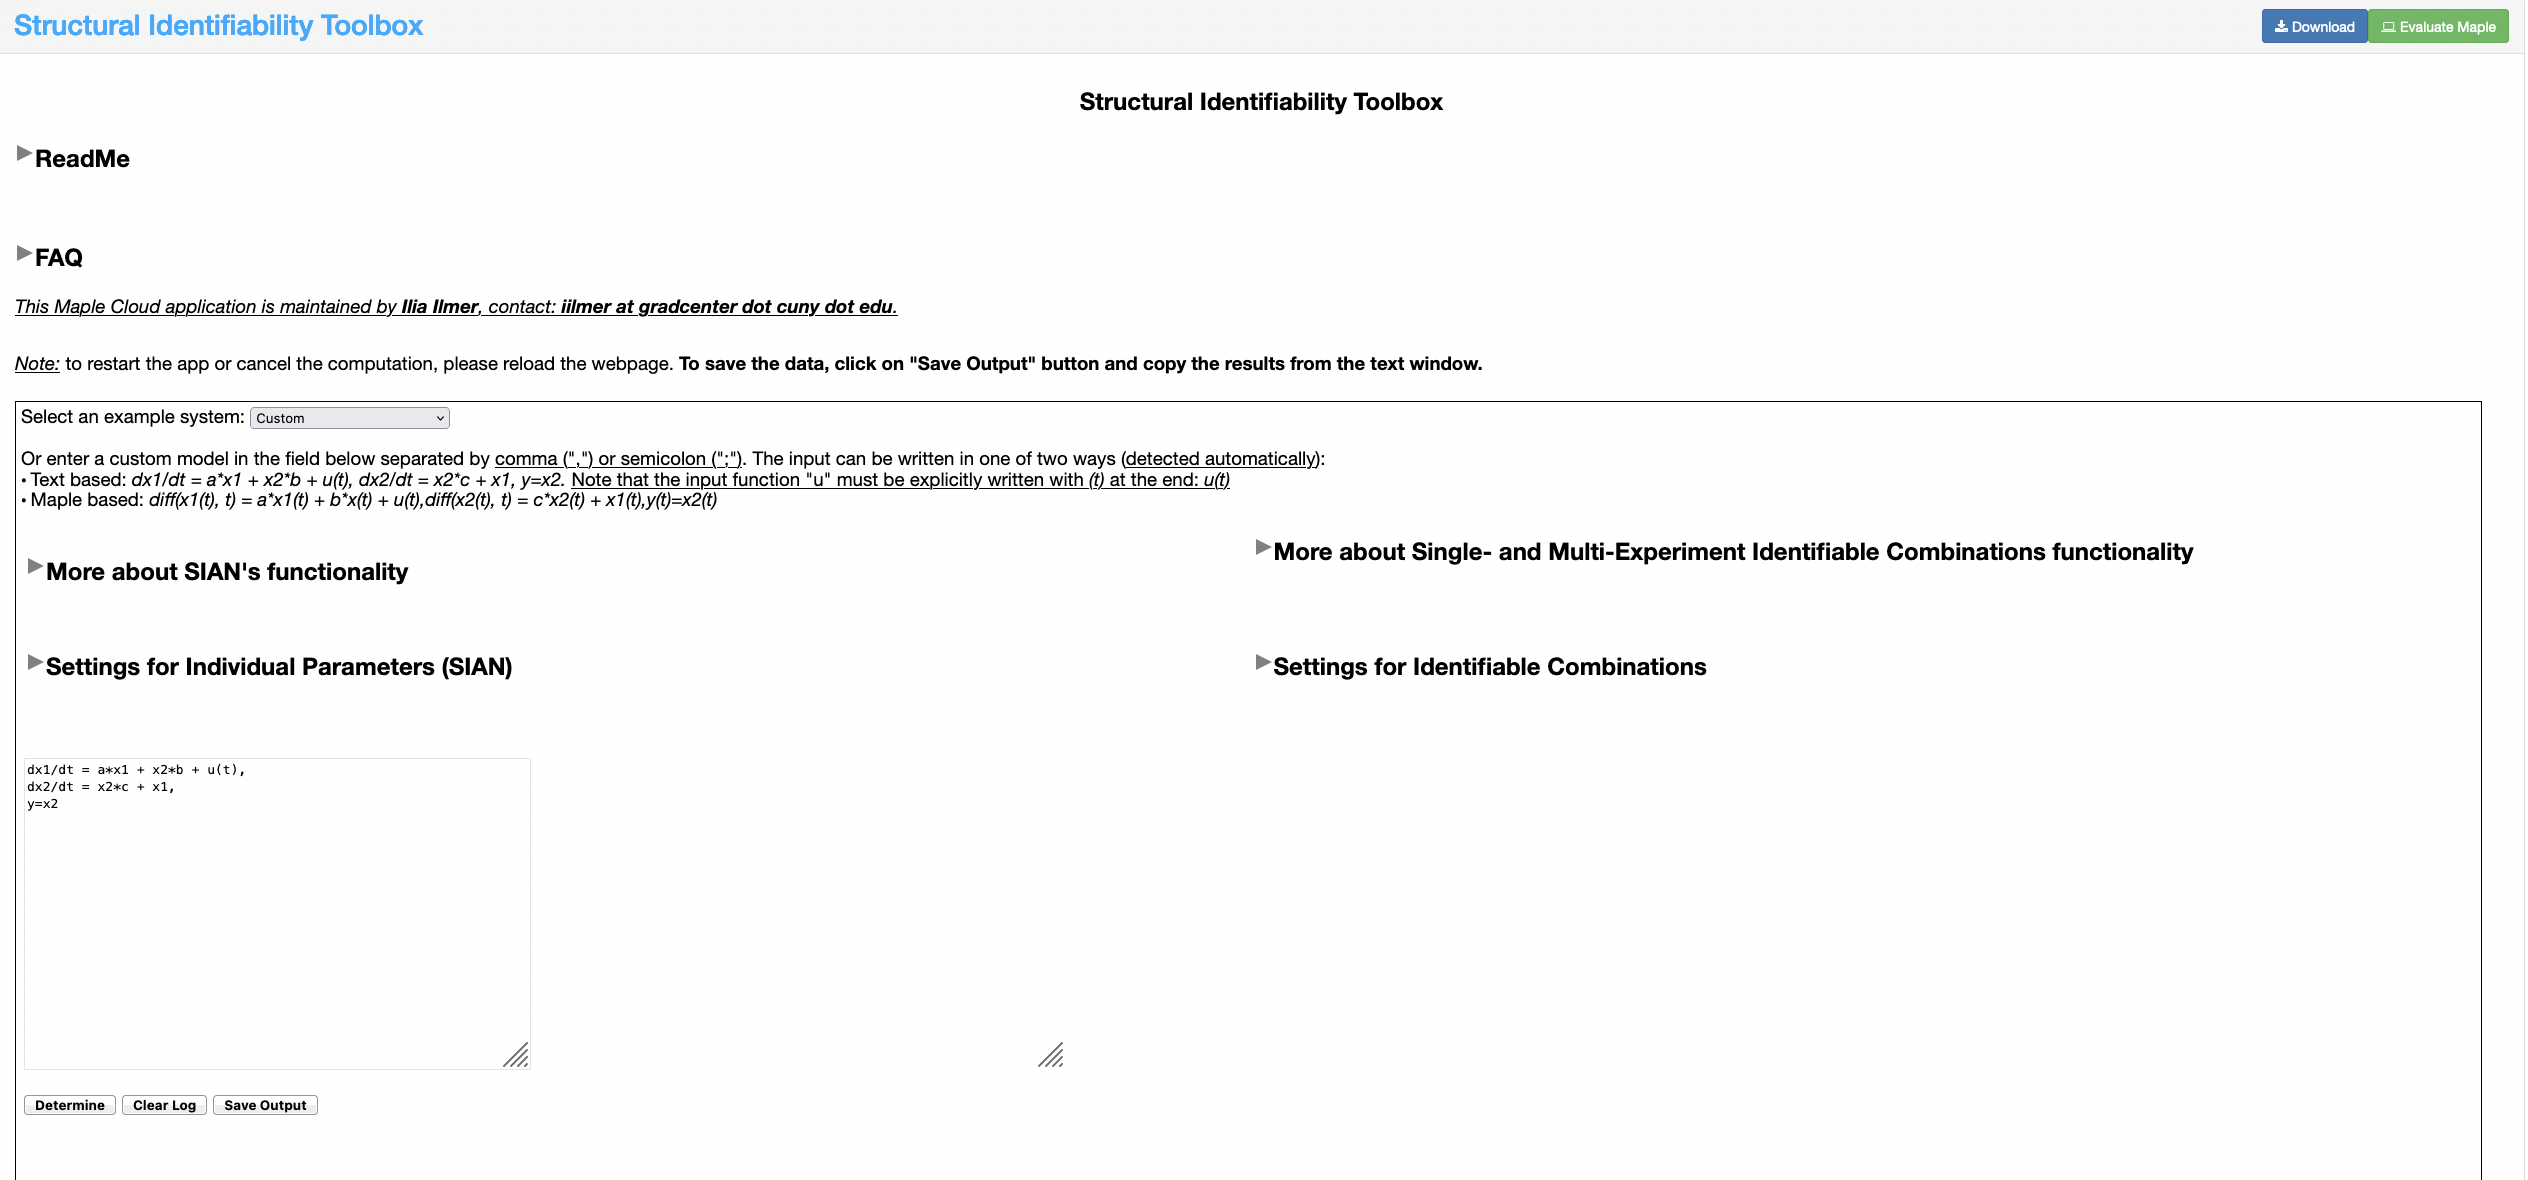
\includegraphics[width=\linewidth]{screenshot.png}
                    \caption{Screenshot of the web-application.}
                \end{figure}

            \end{block}

            %----------------------------------------------------------------------------------------
            %	CONCLUSION
            %----------------------------------------------------------------------------------------

            \begin{block}{Final Remarks}
                Our program provides:
                \begin{itemize}
                    \item Fast identifiability analysis without requiring any installations.
                    \item Low overhead of individual parameter identifiability can accelerate finding identifiable combination.
                \end{itemize}
                Some future work includes:
                \begin{itemize}
                    \item Computing characteristic sets via {\tt DifferentialAlgebra} (\cite{boulier2004blad}) is still an overhead.
                    \item We are investigating differential Thomas decomposition for single- and multi-experiment identifiability problems~\cite{gerdt2019maple}.
                \end{itemize}

            \end{block}

            %----------------------------------------------------------------------------------------
            %	REFERENCES
            %----------------------------------------------------------------------------------------

            \begin{block}{References}

                % \nocite{*} % Insert publications even if they are not cited in the poster
                \small{%\bibliographystyle{unsrt}
                    \printbibliography{}}

            \end{block}

            %----------------------------------------------------------------------------------------
            %	ACKNOWLEDGEMENTS
            %----------------------------------------------------------------------------------------

            \begin{block}{Acknowledgments}

                \begin{itemize}
                    \item The authors are grateful to CCiS at CUNY Queens College. This work was partially supported by the NSF under grants CCF-1563942, CCF-1564132, DMS-1760448, DMS-1853650, and DMS-1853482

                \end{itemize}

            \end{block}

            %----------------------------------------------------------------------------------------
            %	CONTACT INFORMATION
            %----------------------------------------------------------------------------------------

            \setbeamercolor{block title}{fg=black,bg=orange!90} % Change the block title color

            \begin{block}{Contact Information}

                \begin{itemize}
                    \item Web: \href{https://iliailmer.github.io}{https://iliailmer.github.io}
                    \item Email: \href{mailto:iilmer@gradcenter.cuny.edu}{iilmer@gradcenter.cuny.edu}
                          % \item Phone: +1 (000) 111 1111
                \end{itemize}

            \end{block}

            %----------------------------------------------------------------------------------------


        \end{column} % End of the second column

        \begin{column}{.015\textwidth}\end{column} % Empty spacer column

    \end{columns} % End of all the columns in the poster

\end{frame} % End of the enclosing frame

\end{document}